\pagestyle{empty} % Limpa o cabeçalho e o rodapé
\onehalfspacing % Espaçamento entre-linhas de 1,5
% \hyphenpenalty=10000 % To prevent hyphenation
\pretolerance=10000 % To avoif overful lines
%\selectlanguage{english}
\setcounter{ex}{0} % counter for exercises
\selectlanguage{brazilian}
%\pagenumbering{arabic} % Uncomment this line if you want renumber pages for each chapter
\renewcommand{\chaptername}{Tutorial}
\chapter{Dados Moleculares - Alinhamento}\label{tut8}
\rhead{\tiny Instituto de Biociências --USP: BIZ0433 - Inferência Filogenética: Filosofia, Método e Aplicações}
\cfoot{\tiny \cc \ccby \ccsa \href{http://creativecommons.org/licenses/by-sa/4.0/}{Creative Commons Attribution-ShareAlike 4.0 International License}}
%\vspace{5pt}
{\large \sc BIZ0433 - Inferência Filogenética: Filosofia, Método e Aplicações.}\par
%\vspace{10pt}
\par
\minitoc % for table of contents within the chapter
\newpage
\section*{}\addcontentsline{toc}{section}{Objetivo}
\onehalfspacing
\vspace*{5pt}
\begin{center}
\emph{\begin{large}Objetivo\end{large}}\label{tut8:Objetivo}
\vspace{2pt}
\end{center}
%% TEXTO DO RESUMO
O objetivo deste tutorial é apresentar os conceitos associados ao alinhamento múltiplo de sequências nucleotídicas e subsequente análise filogenética. Neste tutorial iremos avaliar os resultados de três programas tradicionalmente utilizados para produzir alinhamentos (Clustalw,Clustal--$\Omega$ Muscle e MAFFT) e alguns dos componentes analíticos comuns a estes programas. Este tutorial requer a execução de uma série de exercícios e a avaliação dos resultados obtidos frente a leitura do artigo de Phillips \textit{et al.} (2000). Ao completar este tutorial, o estudante terá uma visão geral dos algoritmos e estratégias de alinhamento múltiplo disponíveis para análises filogenéticas dentro do conceito de homologia estática, bem como dos problemas associados a esta prática em inferência filogenética. Os arquivos associados a este tutorial estão disponíveis em \url{http://lhe.ib.usp.br/cladistica}. Você pode baixá-los diretamente com o seguinte comando:

\begin{center}
\small \texttt{wget http://lhe.ib.usp.br/downloads/tutorial\_08.zip}\\
\end{center}

\newpage
\pagestyle{fancy} % Inclui o cabeçalho definido no meta.tex
%\pagenumbering{arabic} % Números das páginas em arábicos
\begin{refsection}
\renewcommand*{\finalnamedelim}{\addspace\&\space} % Usar '&' ao invés de 'e'.
%
%% color base pairs
\newcommand{\A}{\textcolor{green}{\textbf{A}}}
\newcommand{\C}{\textcolor{blue}{\textbf{C}}}
\newcommand{\G}{\textcolor{gray}{\textbf{G}}}
\newcommand{\T}{\textcolor{red}{\textbf{T}}}
\newcommand{\gap}{\textcolor{black}{\textbf{-}}}


%%%%%%%%%%%%%%%%%%%%%%%%%%%% HERE TEXT STARTS %%%%%%%%%%%%%%%%%%%%%%%%%%%% 
\section{Contextualização}\label{tut8:context}

A maioria das análises filogenéticas convencionais baseadas em dados moleculares requer um esquema de correspondência entre os pares de base que antecede à buscas de topologias -- ou seja, a análise filogenética propriamente dita \parencite{Wheeler_2012}. Isso decorre da observação de que, em muitos casos, regiões homólogas do genoma diferem em tamanho em consequência da composição diferencial de pares de base. O processo de conversão entre sequências de tamanhos distintos em sequências de mesmo tamanho é chamado de \textit{alinhamento} ou ainda \textit{alinhamento múltiplo}. Considere por exemplo a seguinte observação:


\indent\indent\indent\indent\indent\indent\indent\texttt{taxon1~~~~~\T\T\G\C\A}\\
\indent\indent\indent\indent\indent\indent\indent\texttt{taxon2~~~~~\T\G\G\G\C\C\A}\\
\indent\indent\indent\indent\indent\indent\indent\texttt{taxon3~~~~~\T\G\C\A\A}\\
\indent\indent\indent\indent\indent\indent\indent\texttt{taxon4~~~~~\T\G\G\C\C\A}\\

Um possível esquema de correspondência (\textit{i.e.}, alinhamento) entre os pares de bases das sequências nucleotídica para estes quatro terminais seria:

\texttt{Alinhamento 1}\\
\indent\indent\indent\indent\indent\indent\indent\texttt{taxon1~~~~~\T\T\G\gap\gap\C\A}\\
\indent\indent\indent\indent\indent\indent\indent\texttt{taxon2~~~~~\T\G\G\G\C\C\A}\\
\indent\indent\indent\indent\indent\indent\indent\texttt{taxon3~~~~~\T\G\gap\gap\C\A\A}\\
\indent\indent\indent\indent\indent\indent\indent\texttt{taxon4~~~~~\T\G\G\gap\C\T\A}\\

ou poderia ser:

\texttt{Alinhamento 2}\\
\indent\indent\indent\indent\indent\indent\indent\texttt{taxon1~~~~~\T\gap\T\G\gap\C\A}\\
\indent\indent\indent\indent\indent\indent\indent\texttt{taxon2~~~~~\T\G\G\G\C\C\A}\\
\indent\indent\indent\indent\indent\indent\indent\texttt{taxon3~~~~~\T\G\gap\gap\C\A\A}\\
\indent\indent\indent\indent\indent\indent\indent\texttt{taxon4~~~~~\T\gap\G\G\C\T\A}\\

Observe que estes dois alinhamentos propõem diferentes séries de transformações para os caracteres 2 e 3, portanto assumem hipóteses de identidades históricas \parencite[senso][]{Grant_and_Kluge_2004} distintas. Em consequência disso, estes dois alinhamentos resultam em hipóteses filogenéticas distintas (Figura \ref{tut8:fig:alinhamentos_examples}). A influência dos alinhamentos em hipóteses filogenéticas é conhecido há tempos. \textcite{Morrison_and_Ellis_1997} examinaram esta relação e concluíram que o resultado de análises filogenéticas são mais influenciadas por alinhamentos do que critérios de otimalidade.

%%%%%%%%%%%%%%%%%%%%%%%%%%% FIGURA BIOEDIT EXAMPLE %%%%%%%%%%%%%%%%%%%%%%%%%%%
%  \vspace{-1em}
  \begin{figure}[H]
    %\ffigbox[\FBwidth]
      {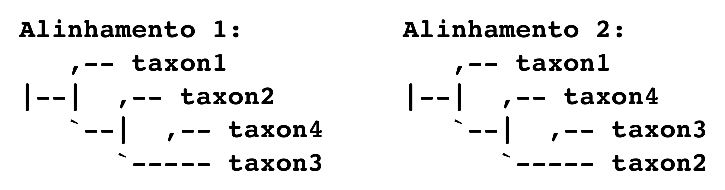
\includegraphics[scale=0.9]{figures/tut8/alinhamentos_examples.eps}}
	{\caption[Consequência de alinhamentos em topologias]{Hipóteses filogenéticas mais parcimoniosas resultantes dos alinhamentos 1 e 2, acima.}\label{tut8:fig:alinhamentos_examples}}
  \end{figure}

%%%%%%%%%%%%%%%%%%%%%%%%%%% FIM DA FIGURA BIOEDIT EXAMPLE %%%%%%%%%%%%%%%%%%%%%

Um dos conceitos mais importantes relacionados aos procedimentos de alinhamento é compreendê-lo como um processo de inferência similar às estimativas de hipóteses filogenéticas. Pares de bases (\textit{i.e.}, \texttt{A}, \texttt{C}, \texttt{G} e \texttt{T}) são observações, mesmo que indiretamente apresentadas pelos cromatogramas de sequenciamento. Os \textit{gaps}, por outro lado, são inseridos durante o processo de alinhamento para traçar as correspondências necessárias -- dentro do contexto de homologia estática \parencite{Wheeler_2001} -- para proceder com a análise filogenética. Igualmente importante é reconhecer que a inserção de \textit{gaps} postulam eventos de inserção e deleções (\textit{i.e.}, \textbf{INDELs}), eventos históricos que consequentemente possuem informação filogenética. Isso é relevante, pois requer que \textit{gaps} sejam tratados como um quinto estado de caráter em análises filogenéticas de sequências nucleotídicas.

Neste tutorial iremos explorar os principais conceitos associados ao procedimento de alinhamento de sequências nucleotídicas. O tutorial seguirá um formato distinto do que vocês estão acostumados até então. Durante o tutorial vocês farão uma série de exercícios cujo objetivo é apresentar a vocês algumas das ferramentas disponíveis para alinhamentos múltiplos, entender os componentes metodológicos associados aos alinhamentos e verificar como as premissas de alinhamento impactam os resultados de análises filogenéticas. No final deste tutorial você encontrará uma série de perguntas que deverão ser respondidas para a próxima aula em referências ao artigo de \textcite{Phillips_et_al_2000}.


\section{Alinhamento, aplicativo e topologias}\label{tut8:msa}

\subsection{Alinhamento manual no Bioedit}\label{tut8:msa:man}

Não é incomum encontrarmos publicações nas quais o alinhamento foi efetuado integralmente ou parcialmente à mão. Os chamados alinhamentos ``\textit{by eye}'' são menos frequentes atualmente, isso é fato, mas seus defensores argumentavam que nosso cérebro era capaz de tomar decisões mais prudentes que os algoritmos disponíveis para essa tarefa. Há uma série de problemas com essa prática que iremos discutir na próxima aula \parencite[veja ][]{Phillips_et_al_2000}. \\


\stepcounter{ex}
\begin{blackBlock}{\textbf{Exercício 8.\arabic{ex}}}\label{tut8:ex:8.1}

Você deverá fazer o alinhamento manual das sequências no arquivo \texttt{seqdata1.fas} utilizando BioEdit. Caso tenha problemas em utilizar esse programa, revise a seção \ref{tut7:handling_files:bioedit} do Tutorial \ref{tut7}. É importante que você tente fazer o melhor alinhamento que considerar possível -- embora devemos reconhecer que a noção de ``melhor'' é extremamente subjetiva --, mas gaste alguns bons minutos ponderando as decisões que o levaram a inserir um \textit{gap} aqui e ali. Após finalizar este alinhamento você deverá salvá-lo sob o nome de ''\texttt{seqdata1\_man.fas}''.

\end{blackBlock}

\subsection{Clustalw}\label{tut8:msa:clustalw}

Um dos aplicativos mais utilizados para alinhamento múltiplo é o Clustalw \parencite{Larkin_et_al_2007}. No Tutorial \ref{tut7} vocês usaram este programa em BioEdit \parencite{Hall_1999}. A documentação do programa pode ser encontrada em \url{http://www.clustal.org/clustal2/} e a documentação das linhas de execução que iremos utilizar estão disponíveis em \url{http://helixweb.nih.gov/multi-align/man/clustalw.1.html}. Não é o objetivo deste tutorial fazer qualquer explanação sobre os algoritmos e estratégias utilizadas pelo Clustalw, mas em \textcite{Phillips_et_al_2000} você encontrará parte dessas informações. O Clustalw está disponível no sistema de vocês. Caso esteja usando uma outra instalação ou sistema operacional, certifique-se que o programa está instalado.


\stepcounter{ex}
\begin{blackBlock}{\textbf{Exercício 8.\arabic{ex}}}\label{tut8:ex:8.2}

Neste exercício você deverá fazer um alinhamento das sequências do arquivo \texttt{seqdata1.fas} utilizando Clustalw. Para fazê-lo, você deverá executar o Clustalw em um terminal utilizando a seguinte linha de comando:\\

\scriptsize
\shellcmd{clustalw -align -output=fasta -outorder=input -infile=seqdata1.fas -outfile=seqdata1\_cltw.fas}\\
\normalsize

\end{blackBlock}


Esta linha de comando, a opção ``\texttt{-align}'' faz com que Clustalw execute o alinhamento múltiplo para as sequências existentes em ``\texttt{-infile=seqdata1.fas}'' obedecendo a ordem dos terminais (``\texttt{-outorder=input}'') quando imprimir os resultados no arquivo de saída ``\texttt{-outfile=seqdata1\_clt.fas}'' no formato ''\texttt{-output=fasta}''. 



\subsection{Clustal--$\Omega$}\label{tut8:msa:clustalo}

Recentemente, \textcite{Sievers_et_al_2011} desenvolveram uma nova versão de Clustal. Chamada de \href{http://www.clustal.org/omega/}{Clusta--Omega} ($\Omega$), esta versão foi considerada mais rápida e ``acurada'' que Clustalw. Dada à sua recente publicação, está versão não é tão popular como a anterior, mas pode ser que isso mude ao longo dos próximos anos.


\stepcounter{ex}
\begin{blackBlock}{\textbf{Exercício 8.\arabic{ex}}}\label{tut8:ex:8.3}

Neste exercício você deverá fazer um alinhamento das sequências do arquivo \texttt{seqdata1.fas} utilizando Clustal-$\Omega$. Para fazê-lo, você deverá executar o Clustal-$\Omega$ em um terminal utilizando a seguinte linha de comando:\\

\scriptsize
\shellcmd{ clustalo {-}{-}full {-}{-}iter=16 -i seqdata1.fas -o seqdata1\_clto.fas -v}\\
\normalsize

\end{blackBlock}

A descrição destas opções pode ser verificada digitando ``\texttt{clustalo {-}{-}help}'' em um terminal ou consultando a doscumentação do programa.


\subsection{Muscle}\label{tut8:msa:muscle}

\href{http://www.drive5.com/muscle/}{Muscle} \parencite{Edgar_2004} é outro aplicativo utilizado para alinhamentos múltiplos. Em termos gerais, esse programa é bem mais rápido que Clustalw, embora menos utilizado na literatura. A forma de alinhamento de Muscle difere razoavelmente de Clustalw. Uma breve explanação sobre estas diferenças é apresentada no \href{http://www.drive5.com/muscle/muscle.html#_Toc81224846}{item 4.1} da documentação de Muscle e não será discutida aqui.\\

\stepcounter{ex}
\begin{blackBlock}{\textbf{Exercício 8.\arabic{ex}}}\label{tut8:ex:8.4}

Neste exercício você irá alinhar as mesmas sequências que alinhou com o Clustalw e Clustal--$\Omega$ utilizando Muscle. Você irá executar o Muscle utilizando seus parâmetros de \textit{default} com a seguinte linha de comando:

\scriptsize
\shellcmd{muscle -in seqdata1.fas -out seqdata1\_mus.fas}\\
\normalsize

\end{blackBlock}

Na linha de comando acima, o arquivo de entrada (\texttt{-in seqdata1.fas}) será alinhado no Muscle e o resultado impresso no arquivo de saída (\texttt{-out seqdata1\_mus.fas}). No entanto,  no arquivo \texttt{-out seqdata1\_mus.fas} a ordem dos terminais está alterada (veja utilizando o comando ``\texttt{less}''). Há uma opção em Muscle para manter a ordem dos terminais idêntica ao arquivo de entrada, porém esta opção (\texttt{-stable}) está com problemas e foi desabilitada nas versões mais recentes do programa. No entanto, o autor disponibilizou um \textit{script} que reordena o alinhamento segundo o arquivo de entrada. Para fazer o mesmo com seus resultados, execute o seguinte comando de linha: 

\scriptsize
\shellcmd{python ./stable.py seqdata1.fas seqdata1\_mus.fas > seqdata1\_mus\_ord.fas}\\
\normalsize

\subsection{Mafft}\label{tut8:msa:mafft}

\href{http://mafft.cbrc.jp/alignment/software/}{MAFFT} \parencite{Katoh_et_al_2002, Katoh_and_Standley_2013} é o último programa que iremos utilizar. Este é um dos programas mais recentes desenvolvidos e possui uma série de algoritmos muito eficientes para gerar alinhamentos. Detalhes sobre tais algoritmos podem ser encontrados nas referências citadas anteriormente ou na página do programa referente aos \href{http://mafft.cbrc.jp/alignment/software/algorithms/algorithms.html}{algoritmos de alinhamento}.\\


\stepcounter{ex}
\begin{blackBlock}{\textbf{Exercício 8.\arabic{ex}}}\label{tut8:ex:8.5}

Neste exercício, você deverá fazer um novo alinhamento das sequências no arquivo ``\texttt{seqdata1.fas}''. Para isso, você deverá executar o MAFFT com a seguinte linha de comando:

\scriptsize
\shellcmd{mafft -{}-maxiterate 1000 -{}-preservecase seqdata1.fas > seqdata1\_mafft.fas}\\
\normalsize

\end{blackBlock}

Na linha de comando acima, o termo ``\texttt{-{}-maxiterate 1000}'' configura o número máximo de iterações que o MAFFT irá usar durante o processo de refinamento do alinhamento das sequências no arquivo de entrada ``\texttt{seqdata1.fas}'' cujo resultado será impresso no arquivo de saída ``\texttt{seqdata1\_mafft.fas}'' preservando as letras maiúsculas dos pares de base de acordo com a opção ``\texttt{-{}-preservecase}''\footnote{ por \textit{default} MAFFT imprime os pares de base em letras minúsculas. Embora para efeitos analíticos isso não importe, letras maiúsculas são desejáveis quando se deseja inspecionar os alinhamentos em programas como BioEdit.}.


\subsection{Avaliação dos resultados}\label{tut8:msa:results}

Ao completarem os exercícios acima, seu diretório de trabalho deverá conter os seguintes aquivos: \texttt{seqdata1\_man.fas}, \texttt{seqdata1\_cltw.fas}, \texttt{seqdata1\_clto.fas}, \texttt{seqdata1\_mus\_ord.fas} e \texttt{seqdata1\_mafft.fas}. Verifique se todos estão presentes e que tenham conteúdo, caso contrário será necessário repetir alguns dos exercícios acima.


\stepcounter{ex}
\begin{blackBlock}{\textbf{Exercício 8.\arabic{ex}}}\label{tut8:ex:8.6}

Sua primeira avaliação será puramente visual. Abra todos os arquivos simultaneamente em BioEdit e responda:

\end{blackBlock}


\begin {myindentpar}{0.3cm}
\begin{enumerate}[\itshape i.]
	\item{Todos os alinhamentos são idênticos?}

\line(1,0){400}\\
\line(1,0){400}\\

\item{Se você tivesse que optar por um desses alinhamentos, qual seria? Justifique sua resposta.}

\line(1,0){400}\\
\line(1,0){400}\\

\item{Abaixo você deverá fazer uma análise filogenética em TNT de todos os alinhamentos gerados (veja Tutorial \ref{tut7} caso não saiba como isso deve ser feito), completar a Tabela \ref{tut8:table:align} e anotar o relacionamento filogenético encontrado em cada uma das análises nos espaços específicos abaixo.}


%%%%%%%%%%%%%%%%%%%%%%%%%%% TABELA DE ANÁLISE DE ALINHAMENTOS %%%%%%%%%%%%%%%%%%%%%%%%%%% 
%\begin{landscape}
\pagestyle{fancy}
\begin{center}

\begin{longtable}{|c|c|c|}
\caption[Análise cladística de vários alinhamentos]{Análise cladística dos alinhamentos gerados por diferentes programas.} \label{tut8:table:align} \\


\hline\hline \textbf{Alinhamento} & \textbf{Número de MPTs}  & \textbf{Custo das MPTs}\\
\endfirsthead

\multicolumn{3}{c}{{\bfseries \tablename\ \thetable{} -- Continuação.}}\\
\hline\hline \textbf{Alinhamento} & \textbf{Número de MPTs} & \textbf{Custo das MPTs}\\
\endhead
%\hline \multicolumn{6}{r}{{--continua na próxima página}} \\ \hline
%\endfoot
\hline \hline
%\hline \multicolumn{6}{l}{Consulte a página \url{http://wiki.linuxquestions.org/wiki/Linux_software_equivalent_to_Windows_software}.}
\endlastfoot

\hline manual &  & \\
\hline Clustalw &  & \\
\hline Clustal-$\Omega$ &  & \\
\hline Muscle &  & \\
\hline MAFFT &  & \\

\end{longtable}
\end{center}
%\end{landscape}
%%%%%%%%%%%%%%%%%%%%%%%%%%% FIM DE ANÁLISE DE ALINHAMENTOS %%%%%%%%%%%%%%%%%%%%%%%%%%

\end{enumerate}
\end{myindentpar}

Topologias encontradas nas análises filogenéticas dos alinhamentos da Tabela \ref{tut8:table:align}:\\

%\begin{center}
%\fbox{\parbox[c][6.5cm][s]{6.5cm}{Manual}}
%\fbox{\parbox[c][6.5cm][s]{6.5cm}{Clustalw}}\\
%\fbox{\parbox[c][6.5cm][s]{6.5cm}{Muscle}}
%\fbox{\parbox[c][6.5cm][s]{6.5cm}{MAFFT}}\\
%\end{center}

\newpage
\section{Parâmetros de alinhamento}\label{tut8:par}

Todos os alinhamentos produzidos pelos programas acima baseiam-se em alinhamentos par a par computados pelo algoritmo de \textcite{Needleman_and_Wunsch_1970}. Este algoritmo está documentado no artigo de \textcite{Phillips_et_al_2000} e depende de parâmetros numéricos que são utilizados no cômputo das distâncias de edição entre duas sequências alinhadas. A distância de edição entre duas sequências é definida pelo número de operações necessárias para tornar uma sequência idêntica a outra. Por exemplo, considere o seguinte alinhamento:

\indent\indent\indent\indent\indent\indent\indent\texttt{taxon1~~~~~\T\A\T\G\gap\gap\A}\\
\indent\indent\indent\indent\indent\indent\indent\texttt{~~~~~~~~~~~~**~**~}\\
\indent\indent\indent\indent\indent\indent\indent\texttt{taxon2~~~~~\T\G\G\G\C\C\A}\\

Observe que são necessárias 4 operações para tornar uma das sequências igual a outra (denotadas com ''\texttt{*}''). Por exemplo, se considerarmos a sequência do \texttt{taxon1} e substituirmos \texttt{\A} por \texttt{\G} na segunda posição, \texttt{\T} por \texttt{\G} na terceira posição e \texttt{\gap} por \texttt{\C} na quinta e sexta posições, as sequências de ambos os terminais tornam-se idênticas. Neste caso, se o custo de cada evento de edição é atribuído a 1, o custo deste alinhamento seria 4. 

Parâmetros de alinhamento podem considerar custos distintos para eventos de edição diferentes -- na expectativa de acomodar algumas premissas associada ao que sabemos sobre evolução molecular. No exemplo acima, a edição necessária na segunda posição envolve um evento de transição (\textit{i.e.}, substituições entre purinas ou pirimidinas), ao passo que na terceira posição o evento de edição envolve uma transversão (\textit{i.e.}, substituições de purina por uma pirimidina, ou vice versa). Em casos como esse, você poderia atribuir custos diferenciais para esses dois tipos de operações de edição. Você poderia ainda levar em consideração que o custo de um \textit{gap} é diferente de dois \textit{gaps} consecutivo. A justificativa para estes custos diferenciais associados à abertura e extensão de \textit{gaps} está no argumento de que INDELs (\textit{i.e.}, inserções e deleções) podem ocorrer em bloco \parencite[mas veja ][]{Giribet_and_Wheeler_1999, Phillips_et_al_2000}.

O cálculo do custo de um alinhamento é necessário por que a função objetiva que cada programa está buscando otimizar depende dele. Todos os programas exemplificados acima tentam maximizar a semelhança entre as sequências alinhadas e, portanto, sua função objetiva minimiza a distância de edição entre elas. Considere o seguinte alinhamento:

\indent\indent\indent\indent\indent\indent\indent\texttt{taxon1~~~~~\T\A\T\G\gap\gap\gap\gap\A}\\
\indent\indent\indent\indent\indent\indent\indent\texttt{~~~~~~~~~~~~**~****~}\\
\indent\indent\indent\indent\indent\indent\indent\texttt{taxon2~~~~~\T\gap\gap\G\G\G\C\C\A}\\

Neste caso, o custo do alinhamento seria 6, maior que o anterior. Mas isso só é verdade se assumirmos que qualquer operação de edição possui o mesmo custo, no caso 1. No entanto, considere custos diferenciais para abertura e extensão de \textit{gap}, no qual o primeiro \textit{gap} recebe valor igual a 1 e os demais 0.5. Neste caso ambos alinhamentos teriam custo igual a 3,5. Adicionalmente, consideremos custos diferenciais para transições e transversões, por exemplo 1 e 2, respectivamente. Neste caso, o primeiro exemplo teria custo igual a 4,5 ao passo que o segundo permaneceria com custo igual a 3,5 -- pois nenhuma operação de edição neste último alinhamento requer substituição entre pares de base. O que fizemos acima foi variar os chamados \textbf{parâmetros de custo} de alinhamentos, e como se observa, eles influenciam o resultado da função objetiva e portanto pode selecionar alinhamentos distintos.

\subsection{Manipulação de parâmetros em MAFFT}\label{tut8:par:op}

Para verificar as relações entre parâmetros de alinhamento e inferência filogenética iremos manipular dois parâmetros disponíveis em MAFFT para 4 alinhamentos distintos e posteriormente fazer uma análise cladística destes alinhamentos.\\


\stepcounter{ex}
\begin{blackBlock}{\textbf{Exercicio 8.\arabic{ex}}}\label{tut8:ex:8.7}

O parâmetro ``\texttt{-{}-op}'' define o que é conhecido como \textit{gap open penalty} em programas de alinhamento e o parâmetro ``\texttt{-{}-ep}'' define o custo de extensão de \textit{gaps}. Em MAFFT, esses parâmetros recebem os valores de 1.53 e 0.123, respectivamente. Obedecendo a sintaxe das linhas de comando abaixo, você deverá produzir 4 alinhamentos distintos, sendo que para um deles será considerado os valores de \textit{default} para estes parâmetros. Para os demais serão atribuídos custos diferentes, porém idênticos para ``\texttt{-{}-op}'' e ``\texttt{-{}-ep}''. Os comandos de linha para a execução destes alinhamentos são as seguintes:\\

\scriptsize
\shellcmd{mafft -{}-maxiterate 1000 -{}-preservecase seqdata2.fas > seqdata2.d.fas}\\
\indent\shellcmd{mafft -{}-op 1 -{}-ep 1 -{}-maxiterate 1000 -{}-preservecase seqdata2.fas > seqdata2.1.fas}\\
\indent\shellcmd{mafft -{}-op 2 -{}-ep 2 -{}-maxiterate 1000 -{}-preservecase seqdata2.fas > seqdata2.2.fas}\\
\indent\shellcmd{mafft -{}-op 3 -{}-ep 3 -{}-maxiterate 1000 -{}-preservecase seqdata2.fas > seqdata2.3.fas}\\
\normalsize

Após gerar estes alinhamentos, você deverá fazer uma análise filogenética destes dados alinhados e anotar os resultados na Tabela \ref{tut8:table:par} e no campo disponível para ilustrar as topologias obtidas, abaixo

\end{blackBlock}

\newpage
%%%%%%%%%%%%%%%%%%%%%%%%%%% TABELA DE ANÁLISE DE PARÂMETROS ALINHAMENTOS %%%%%%%%%%%%%%%%%%%%%%%%%%% 
%\begin{landscape}
\pagestyle{fancy}
\begin{center}

\begin{longtable}{|c|c|c|}
\caption[Efeito de parâmetros de alinhamento em inferência filogenética]{Efeito de parâmetros de alinhamento em inferência filogenética para as sequências do arquivo \texttt{seqdata2.fas}.} \label{tut8:table:par} \\


\hline\hline \textbf{Alinhamento} & \textbf{Número de MPTs}  & \textbf{Custo das MPTs}\\
\endfirsthead

\multicolumn{3}{c}{{\bfseries \tablename\ \thetable{} -- Continuação.}}\\
\hline\hline \textbf{Alinhamento} & \textbf{Número de MPTs} & \textbf{Custo das MPTs}\\
\endhead
%\hline \multicolumn{6}{r}{{--continua na próxima página}} \\ \hline
%\endfoot
\hline \hline
%\hline \multicolumn{6}{l}{Consulte a página \url{http://wiki.linuxquestions.org/wiki/Linux_software_equivalent_to_Windows_software}.}
\endlastfoot

\hline \textit{default} &  & \\
\hline \texttt{-{}-op 1} &  & \\
\hline \texttt{-{}-op 2} &  & \\
\hline \texttt{-{}-op 3} &  & \\

\end{longtable}
\end{center}
%\end{landscape}
%%%%%%%%%%%%%%%%%%%%%%%%%%% FIM DA TABELA DE ANÁLISE DE PARÂMETROS ALINHAMENTOS %%%%%%%%%%%%%%%%%%%%%%%%%%


Topologias encontradas nas análises filogenéticas sob diferentes parâmetros de alinhamento da Tabela \ref{tut8:table:par}:

\begin{center}
\fbox{\parbox[c][6.5cm][s]{6.5cm}{\textit{default}}}
\fbox{\parbox[c][6.5cm][s]{6.5cm}{\texttt{-{}-op 1}}}\\
\fbox{\parbox[c][6.5cm][s]{6.5cm}{\texttt{-{}-op 2}}}
\fbox{\parbox[c][6.5cm][s]{6.5cm}{\texttt{-{}-op 3}}}\\
\end{center}

\section{Alinhamento progressivo e árvores-guias}\label{tut8:guide_tree}

O algoritmo de Needleman-Wunsch \parencite{Needleman_and_Wunsch_1970}, utilizado pela maioria dos aplicativos de alinhamento múltiplo, foi concebido para alinhar pares de sequências. Desta forma, ele é bidimensional. Por esta razão, para que os chamados alinhamentos múltiplos sejam executados pelo alinhamento par a par das sequências envolvidas é necessário definir quais seriam os pares alinhados para que ao final tivéssemos um alinhamento completo de todas as sequências de interesse. Todos os programas selecionam pares, sejam eles de táxons terminais (OTUs) ou de vértices internos (HTUs) de acordo com o que denominamos de árvore-guia (\textit{i.e., guide trees}). Estas árvores-guias são geradas, via de regra, na fase inicial do alinhamento \parencite[consulte ][]{Phillips_et_al_2000} e determinam a ordem progressiva dos pares que serão submetidos ao algoritmo de Needleman-Wunsch. O resultado final é o chamado ``alinhamento múltiplo''.

\subsection{Examinando a influência de diferentes árvores-guias em alinhamentos múltiplos}\label{tut8:guide_tree:trees}

Neste componente do tutorial iremos examinar como árvores-guias influenciam os alinhamentos. Iremos considerar quatro árvores-guias para as sequências do arquivo \texttt{seqdata2.fas}\footnote{ os comandos de linha para obtenção e controle da árvores-guias em MAFFT estão disponíveis em \url{http://mafft.cbrc.jp/alignment/software/treein.html} e \url{http://mafft.cbrc.jp/alignment/software/treeout.html}.} (Figura \ref{tut8:fig:guide_trees}).\\

%%%%%%%%%%%%%%%%%%%%%%%%%%% FIGURA BIOEDIT EXAMPLE %%%%%%%%%%%%%%%%%%%%%%%%%%%
%  \vspace{-1em}
  \begin{figure}[h!]
    %\ffigbox[\FBwidth]
      {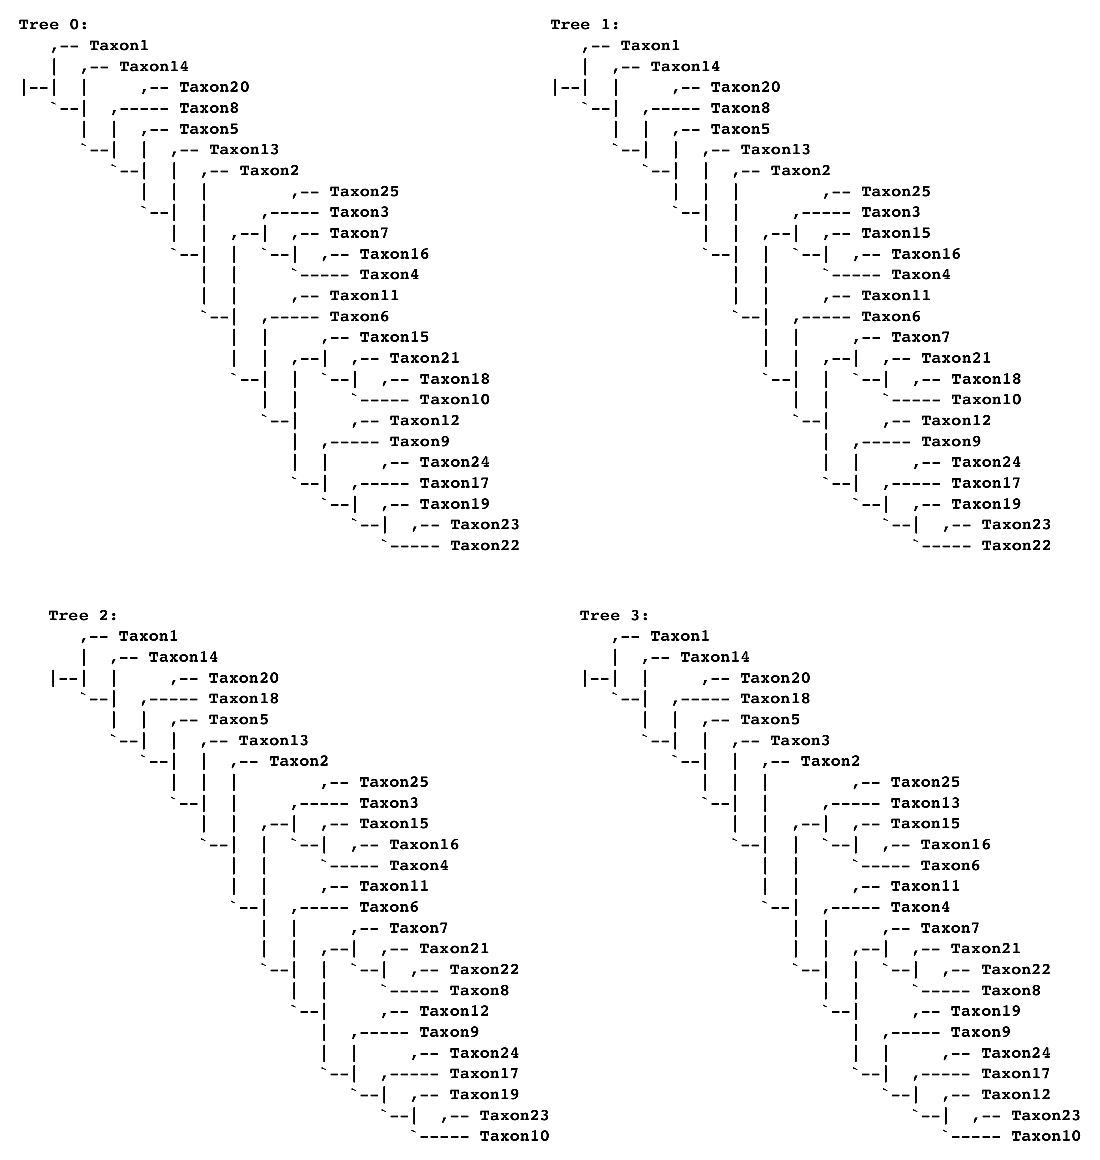
\includegraphics[scale=0.6]{figures/tut8/guide_trees.eps}}
	{\caption[árvores-guias]{Quatro árvores-guias utilizadas no Exercício 8.8 para verificar o efeito dessas topologias nos alinhamentos múltiplos. Estas topologias estão nos arquivos \texttt{new\_guide\_*.tre} e foram transformados para o formato compatível com MAFFT nos arquivos \texttt{new\_guide\_tree*.mafft}.}\label{tut8:fig:guide_trees}}
  \end{figure}

%%%%%%%%%%%%%%%%%%%%%%%%%%% FIM DA FIGURA BIOEDIT EXAMPLE %%%%%%%%%%%%%%%%%%%%%



\stepcounter{ex}
\begin{blackBlock}{\textbf{Exercicio 8.\arabic{ex}}}\label{tut8:ex:8.8}

Você deverá executar as linhas de comando abaixo, cada uma delas irá alinhar as sequências do arquivo \texttt{seqdata2.fas} considerando cada uma das árvores-guias disponíveis nos arquivos \texttt{new\_guide\_tree*.mafft}:\\

\scriptsize
\shellcmd{mafft -{}-maxiterate 1000 -{}-preservecase seqdata2.fas > seqdata2.d.fas}\\
\indent\shellcmd{mafft  -{}-op 1  -{}-ep 1  -{}-treein new\_guide\_tree0.mafft  -{}-maxiterate 1000  -{}-preservecase seqdata2.fas > seqdata2.1.0.fas}\\
\indent\shellcmd{mafft  -{}-op 1  -{}-ep 1  -{}-treein new\_guide\_tree1.mafft  -{}-maxiterate 1000  -{}-preservecase seqdata2.fas > seqdata2.1.1.fas}\\
\indent\shellcmd{mafft  -{}-op 1  -{}-ep 1  -{}-treein new\_guide\_tree2.mafft  -{}-maxiterate 1000  -{}-preservecase seqdata2.fas > seqdata2.1.2.fas}\\
\indent\shellcmd{mafft  -{}-op 1  -{}-ep 1  -{}-treein new\_guide\_tree3.mafft  -{}-maxiterate 1000  -{}-preservecase seqdata2.fas > seqdata2.1.3.fas}\\
\normalsize

Após gerar estes alinhamentos, você deverá fazer uma análise filogenética destes dados alinhados e anotar os resultados na Tabela \ref{tut8:table:guide_tree} e no campo disponível para ilustrar as topologias obtidas, abaixo.

\end{blackBlock}


%%%%%%%%%%%%%%%%%%%%%%%%%%% TABELA DE ANÁLISE DE PARÂMETROS ALINHAMENTOS %%%%%%%%%%%%%%%%%%%%%%%%%%% 
%\begin{landscape}
\pagestyle{fancy}
\begin{center}

\begin{longtable}{|c|c|c|}
\caption[Efeito de árvore-guia em inferência filogenética]{Efeito de árvore-guia em inferência filogenética para as sequências do arquivo \texttt{seqdata2.fas}.} \label{tut8:table:guide_tree} \\


\hline\hline \textbf{Árvore-guia} & \textbf{Número de MPTs}  & \textbf{Custo das MPTs}\\
\endfirsthead

\multicolumn{3}{c}{{\bfseries \tablename\ \thetable{} -- Continuação.}}\\
\hline\hline \textbf{Alinhamento} & \textbf{Número de MPTs} & \textbf{Custo das MPTs}\\
\endhead
%\hline \multicolumn{6}{r}{{--continua na próxima página}} \\ \hline
%\endfoot
\hline \hline
%\hline \multicolumn{6}{l}{Consulte a página \url{http://wiki.linuxquestions.org/wiki/Linux_software_equivalent_to_Windows_software}.}
\endlastfoot

\hline \texttt{new\_guide\_0.tre} &  & \\
\hline \texttt{new\_guide\_1.tre} &  & \\
\hline \texttt{new\_guide\_2.tre} &  & \\
\hline \texttt{new\_guide\_3.tre} &  & \\

\end{longtable}
\end{center}
%\end{landscape}
%%%%%%%%%%%%%%%%%%%%%%%%%%% FIM DA TABELA DE ANÁLISE DE PARÂMETROS ALINHAMENTOS %%%%%%%%%%%%%%%%%%%%%%%%%%


\newpage
Topologias encontradas nas análises filogenéticas utilizando diferentes árvores-guias:

\begin{center}
\fbox{\parbox[c][9.5cm][s]{6.5cm}{\texttt{new\_guide\_0.tre}}}
\fbox{\parbox[c][9.5cm][s]{6.5cm}{\texttt{new\_guide\_1.tre}}}\\
\fbox{\parbox[c][9.5cm][s]{6.5cm}{\texttt{new\_guide\_2.tre}}}
\fbox{\parbox[c][9.5cm][s]{6.5cm}{\texttt{new\_guide\_3.tre}}}\\
\end{center}

\section{Consistência interna da análise}\label{tut8:consistency}

As análise executadas até o momento sofrem de pelo menos duas inconsistências analíticas severas. A primeira delas está relacionada ao fato de que os algoritmos utilizados para criar as árvores-guias possuem uma função objetiva completamente diferente daquela que você utilizou nas análises filogenéticas. Todas as árvores-guias geradas pelos programas de alinhamento múltiplo que utilizamos até o momento são geradas por algoritmos fenéticos, para os quais a função objetiva minimiza a distância fenética entre as sequências. Desta forma, árvores-guias em Clustalw, Clustal-$\Omega$, Muscle e MAFFT são fenogramas. No entanto, ao analisarmos os alinhamentos em TNT, nós abandonamos esse critério de otimalidade (distância fenética) e adotamos outro (distância patrística de série de transformações por parcimônia)! Não seria prudente epistemologicamente manter a consistência da função objetiva, e consequentemente critério de otimalidade, ao longo de toda a análise? A segunda inconsistência analítica refere-se ao fato de que os parâmetros dos parâmetros de custos de alinhamento, escolhidos de arbitrariamente -- diga-se de passagem --, foram ignorados durante a etapa de inferência filogenética. Desta forma, você utilizou uma série de premissas para gerar os dados que foram desconsideradas no memento em que você utilizou estes mesmos dados para inferir relações de parentesco. O MAFFT, por exemplo, utiliza uma razão de 2:1 para transversões e transições que não foi considerada quando você fez uma análise cladística daquele alinhamento. O mesmo pode ser dito para todas as análises do Exercício 8.7. Em todos esses casos, as premissas analíticas não foram consistentes ao longo de todas as etapas de sua análise.

\subsection{Consistência de premissas de alinhamento}\label{tut8:consistency:par}

Quando se adota programas como Clustalw, Clustal-$\Omega$, Muscle e MAFFT não é possível manter consistência dos critérios de otimização -- assumindo que sua análise filogenética não utilize métodos fenéticos. Se seu critério de otimalidade em inferência filogenética é parcimônia, é necessário utilizar programas como, por exemplo, MALIGN \parencite{Wheeler_and_Gladstein_1994} para manter a consistência interna da análise. Seja como for, o que iremos fazer a seguir é minimizar estas inconsistências analíticas implementando as premissas de custo de alinhamento em análises filogenéticas.

Para manter as premissas de alinhamento durante a análise filogenética é preciso implementar as mesmas funções de custo atribuídas para os abertura e extensão de \textit{gaps} e também custos diferenciais de transformação durante o alinhamento na análise filogenética. MAFFT atribui penalidades distintas para transversões e transições na razão de 2:1, respectivamente. Nas análises do Exercício 8.7, nós atribuímos custos diferentes dos parâmetros de \textit{default} do programa para os \textit{gaps}. A implementação dessas premissas em TNT é feita por matrizes de Sankoff. Consulte o a seção \ref{tut6:chartypes} do Tutorial \ref{tut6} para relembrar como caracteres de Sankoff são implementados em TNT.\\

\stepcounter{ex}
\begin{blackBlock}{\textbf{Exercício 8.\arabic{ex}}}\label{tut8:ex:8.9}

Sua tarefa é implementar as premissas de alinhamento na reanálise das sequências dos arquivos \texttt{seqdata2.2.fas} e \texttt{seqdata2.3.fas} produzidas no Exercício 8.7 deste tutorial. Os resultados dessas análises devem ser compilados na Tabela \ref{tut8:table:implement} e nos campos abaixo.

\end{blackBlock}




%%%%%%%%%%%%%%%%%%%%%%%%%%% TABELA DE ANÁLISE DE PARÂMETROS ALINHAMENTOS %%%%%%%%%%%%%%%%%%%%%%%%%%% 
%\begin{landscape}
\pagestyle{fancy}
\begin{center}

\begin{longtable}{|c|c|c|}
\caption[Implementação dos parâmetros de alinhamento em análises filogenéticas]{Implementação dos parâmetros de alinhamento em análises filogenéticas.} \label{tut8:table:implement} \\


\hline\hline \textbf{Dados} & \textbf{Número de MPTs}  & \textbf{Custo das MPTs}\\
\endfirsthead

\multicolumn{3}{c}{{\bfseries \tablename\ \thetable{} -- Continuação.}}\\
\hline\hline \textbf{Dados} & \textbf{Número de MPTs} & \textbf{Custo das MPTs}\\
\endhead
%\hline \multicolumn{6}{r}{{--continua na próxima página}} \\ \hline
%\endfoot
\hline \hline
%\hline \multicolumn{6}{l}{Consulte a página \url{http://wiki.linuxquestions.org/wiki/Linux_software_equivalent_to_Windows_software}.}
\endlastfoot

\hline \texttt{seqdata2.2.fas} &  & \\
\hline \texttt{seqdata2.3.fas} &  & \\

\end{longtable}
\end{center}
%\end{landscape}
%%%%%%%%%%%%%%%%%%%%%%%%%%% FIM DA TABELA DE ANÁLISE DE PARÂMETROS ALINHAMENTOS %%%%%%%%%%%%%%%%%%%%%%%%%%


Topologias encontradas nas análises filogenéticas para as quais você implementou as premissas de alinhamento durante a análise filogenética:

\begin{center}
\fbox{\parbox[c][10.5cm][s]{6.5cm}{\texttt{seqdata2.2.fas}}}
\fbox{\parbox[c][10.5cm][s]{6.5cm}{\texttt{seqdata2.3.fas}}}\\
\end{center}



%%%%%%%%%%%%%%%%%%%%% HERE STARTS QUESTIONS RELATED TO THE TUTORIAL EXCERCISES %%%%%%%%%%%%%%%%%%%%%
\newpage
\section{Questões}\label{tut8:quiz}

\begin {myindentpar}{0.5cm}
\begin{enumerate}[\itshape 1.]

	\item{Você tem alguma objeção ao uso de alinhamentos manuais? Comente.}

\line(1,0){400}\\
\line(1,0){400}\\
\line(1,0){400}\\
\line(1,0){400}\\

	\item{Os resultados dos exercícios da seção \ref{tut8:msa} lhe permitem identificar algum critério objetivo que possa ser usado para a seleção de algum dos alinhamentos que você produziu? Justifique.}

\line(1,0){400}\\
\line(1,0){400}\\
\line(1,0){400}\\
\line(1,0){400}\\
\line(1,0){400}\\
\line(1,0){400}\\


	\item{Parâmetros de alinhamento influenciam reconstruções filogenéticas? Comente de acordo com os resultados que você obteve nos exercícios acima.}

\line(1,0){400}\\
\line(1,0){400}\\
\line(1,0){400}\\
\line(1,0){400}\\

	\item{Você considera que esses parâmetros de alinhamento são arbitrários? Justifique.}

\line(1,0){400}\\
\line(1,0){400}\\
\line(1,0){400}\\
\line(1,0){400}\\


	\item{Árvores-guias influenciam o resultado final do alinhamento? Comente de acordo com os resultados que você obteve nos exercícios acima..}

\line(1,0){400}\\
\line(1,0){400}\\
\line(1,0){400}\\
\line(1,0){400}\\

	\item{Dentre as árvores-guias exploradas no Exercício 8.8, alguma(s) dela(s) gerou(am) um alinhamento que você consideraria melhor do que aqueles obtidos até o momento para as sequências do arquivo \texttt{seqdata2.fas}? Justifique.}

\line(1,0){400}\\
\line(1,0){400}\\
\line(1,0){400}\\

	\item{A topologia da árvores-guias nos exercícios que você fez diferem daquelas obtidas pelas análises filogenéticas das sequências alinhadas? Por que você acha que isso ocorre?}

\line(1,0){400}\\
\line(1,0){400}\\
\line(1,0){400}\\
\line(1,0){400}\\


	\item{A implementação dos premissas de custo de alinhamento durante a análise filogenética modificou os resultados que você havia obtido até então para esses dados? Comente de acordo com os resultados que você obteve nos exercícios acima.}

\line(1,0){400}\\
\line(1,0){400}\\
\line(1,0){400}\\
\line(1,0){400}\\
\line(1,0){400}\\
\line(1,0){400}\\
\line(1,0){400}\\

\end{enumerate}
\end{myindentpar}


\section{Leitura recomendada para discutir seus resultados}\label{tut8:reading}

\fullcite{Phillips_et_al_2000}\\


%%%%%%%%%%%%%%%%%%%%%%%%%%%% HERE ENDS TEXT AND ADDS REFERENCES %%%%%%%%%%%%%%%%%%%%%%%%%%%% 
\section{Referências}\label{tut8:refs}
\printbibliography[heading=none]
\end{refsection}
%  
